\section{Parcial con respecto a los pesos en la última capa}

\begin{figure}[H]
 \centering
 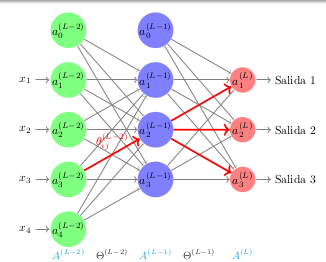
\includegraphics[scale=0.8]{../Figuras/AredN.png}
 %\caption{última capa.}
 \label{fig:graficaLog}
\end{figure}


En esta sección vamos trabajar con la última capa, vamos a tener un poco más de elementos pero va a ser sencillo agregarlos en primer lugar vamos a tener que observar quienes se ven afectados por el nuevo peso con respecto al cual queremos derivar bien aquí tenemos un poco más de transmisión de efecto este peso solamente afecta a esta neurona pero a través de esta neurona ahora si estamos conectados con absolutamente todas las otras neuronas entonces aquí vamos a tener que hacer los toman en cuenta más términos clientes para poder hacer esta derivación voy a tener que volver a empezar desde un principio es decir vamos a volver a empezar con la función de error original y vamos a tener que empezar a derivar desde aquí vamos a recordar ahora que cada vez que calculamos los valores de activación en la última capa bueno estos provienen en realidad también dependen de el valor de activación en esta neurona de acá atrás entonces eventualmente vamos a tener que regresar hasta acá y el valor de esta neurona pues dependió ahora sí directamente del peso que nos está interesando entonces vamos a ir desarrollando poco a poco esa composición de funciones entonces comencemos con el mismo paso de antes calculamos la derivada parcial de jota con respecto al peso correspondiente pero ahora si no puedo eliminar la suma que tengo al inicio porque todos los valores de salida dependen de el peso con el que estamos trabajando entonces lo que vamos a tener aquí ahorita es que nos quedamos con la suma lo único que estoy haciendo ahora es pasarla junto con el signo menos recordemos que la derivada de una suma es la suma de las derivadas entonces podemos meter inmediatamente nuestro problema de derivar a la parte de adentro y simplemente dejar la suma que fuera entonces la primera parte se ve idéntica que antes esto es una constante derivada del logaritmo eso no entre acá para poder calcular esta parcial entonces tenemos que recordar como estaba escrita y lo mismo va a ocurrir de este lado va a salir del signo menos por lo que teníamos acá adentro y tenemos entonces 1 - entre 1 - acá por la parcial de estar acá es lo que estamos sustituyendo acá ya hicimos todas las cuentas todo lo que se cancela entonces no es necesario volverlo a hacer simple y sencillamente llegamos a lo que ya teníamos antes era ye menos llega a menos acá todo esto a lo que se le había llamado delta acá y lo que vamos a empezar ahora es a sacar un poquito los detalles estábamos antes derivando con respecto antes de vestido con respecto a jk y solamente nos había quedado un término aquí en este caso estamos derivando con respecto a y jota y quien depende de y jota pues son las as es básicamente estos pesos son constantes cuando los consideramos con respecto a este que nos interesa ahora y como ahora pues recordamos que nuestra en red está siendo alimentada por todos estos caminos lo que vamos a tener es que por cada uno de estos términos si no se está sobreviviendo el peso que acompaña a esta j entonces por eso aquí vamos a tener nuestro término delta que a pues está acompañado por el respectivo peso que conecta a la neurona o está con la neurona que sale acá y ahora lo que tenemos que hacer es calcular la parcial de este valor de activación la buena noticia es que efectivamente solamente nos interesa un valor de activación que es el de esta neurona jsm que es con la que nos estamos conectando todos los demás en este momento no nos van a afectar pero entonces de aquí están saliendo precisamente estos términos y ahora para poder calcular esta derivada parcial pues vamos a repetir lo mismo de antes que es recordar cómo fue calculada y ahí es donde va a aparecer ahora si explícitamente el peso y jota que es el que nos interesa bien para ir simplificando el bueno de este paso para este paso simple y sencillamente se hace en la sustitución ahora vamos a estar trabajando sobre la siss que serían todas estas neuronas de acá que fueron las que contribuyeron con sus distintos pesos a poder calcular este valor este que está aquí entonces sería la combinación lineal esta neurona por eso le pusimos aquí el índice j y ahora lo que vamos a tratar de hacer es ir simplificando poco a poco esta notación entonces ahora sí vamos a aprovechar que esto se llama delta acá y aquí lo que tenemos es la misma suma pero de esto escribimos delta acá y este es exactamente el mismo peso que estamos colocando acá de aquí bueno regla de la cadena recordemos las propiedades que tienen gente simplemente dejamos indicado que prima con respecto a z j sería que prima evaluado en z j y la derivada de lo que está acá dentro de lo que esté que dentro ahora sí a diferencia de este caso donde nos quedamos con varios pesos en este solamente hay uno que es el que basa un elemento que va a sobrevivir estamos derivando con respecto a y j entonces ahora las variables son éstas las que están en que son las constantes y solamente hay una es cuando y vale exactamente ahí y cuando calcula la derivada con respecto a sí misma pues va a ser 1 y sobrevive una desde toda esta suma solamente sobrevive precisamente ahí es la que tenemos aquí entonces aquí está está ahí que sobrevivió a todo este elemento que tenemos aquí de hecho observemos que cómodamente está ahí no depende del acá realmente si la podemos actualizar a todo esto y le íbamos a llamar del pj y entonces podemos reescribir ahora si nuestras ecuaciones de manera un poco más cómoda ya teníamos entonces de la primera capa que el error cometido por la última capa lo podíamos ver directamente como la diferencia entre lo que queríamos y lo que logramos calcular esto tiene una característica bastante interesante es exactamente por cada neurona tenemos uno de estos después venía la parcial de j con respecto a cada uno de los pesos observemos que por cada uno de estos errores vamos a tener de hecho tantos componentes de éstas como pesos estaban conectados con la carísima neurona entonces de estos tenemos un montón y lo único que teníamos que hacer era multiplicar este valor único por el valor de activación de la neurona con la cual estaba conectado y bueno aquí el signo menos que venimos cargando por la definición de la función de error y ya está ahora equipo se ve con estas tres neuronas bien en la definición de este delta j donde tenemos un producto de las delta casa que venían capa que está más hacia adelante multiplicados por los pesos correspondientes tenemos una suma sobre todos los elementos en última capa y una vez que hicimos esto viene multiplicar por función prima evaluada en la receta j observemos una vez más que está nada más depende de jota no depende de las casas entonces por eso lo podríamos poner entonces realmente le suma nada más afecta este ya que tenemos entonces este producto este que está aquí.
Otra vez tenemos uno por cada neurona en la capa de en medio entonces aquí tenemos las casas aunque vamos a tener las jotas y tenemos uno por cada una de estas este se suele interpretar también como la contribución el error o el error que cometieron todas las neuronas en la capa de enmedio y observen que el error de cada neurona pues realmente tiene una es la suma de como contribuyó al error de todas las neuronas que estaban en la capa siguiente pues tiene mucho sentido no se están participando en todos lados pues su error es la suma de todos los errores a los cuales contribuyó y entonces para calcular el gradiente otra vez nos queda una fórmula bastante sencilla es multiplicar este único error por el valor de activación de la neurona con la cual estaba conectada en la capa anterior y de esta manera podemos obtener todas las parciales con respecto a los pesos que estaban conectados con estas neuronas y aquí tenemos todos esos y este que quedaría la parte de hacer el cálculo directamente el siguiente problema que vamos a tener es bueno si podríamos implementar perfectamente ya con un algoritmo de descenso por el gradiente con estas fórmulas que tenemos aquí simplemente tendremos un montón de ciclos fort para estar calculando todas estas sumas y multiplicaciones sin embargo la forma en la que se acostumbra a trabajar ahora con las redes neuronales no es directamente calculando esto componente por componente sino que lo vamos a utilizar connotación matricial esto va a tener varias ventajas por un lado la notación va a ser muchísimo más compacta y por otro lado va a permitir en la implementación de los algoritmos con procesadores como duda lineal con gpu a piece como q da para procesadores con gpu de manera que estas operaciones se están realizando en paralelo y entonces trabajamos muchísimo más rápido con las redes neuronales y realmente el estar utilizando notación matricial va a tener un impacto directo sobre el tiempo que tardan en ejecutarse nuestros algoritmos y aquellos que están preocupados un poco por la ecología nos dirán que si tardaremos poco tiempo pero vamos a estar gastando muchísima electricidad.
